\documentclass{article}
\usepackage[utf8]{inputenc}
\usepackage[T1]{fontenc}
\usepackage{graphicx}
\usepackage{hyperref}
\usepackage{geometry}
\geometry{margin=1in}

\title{THILSPH}
\date{Encyclopaedia Britannica (1771)}

\begin{document}
\maketitle

\section*{Historical source}
\textbf{Entry ID:} \texttt{entry-thilsph-1614} \\
\textbf{Volume ID:} 144133903 \\
\textbf{Character Count:} 2441

\subsection*{Extracted Text}
THILSPH, in botany, a genus of the térdrynania filicul lofa clais. The pod is emarginated, heart-shaped, containing many feeds. There are ten species, for of them native of Britain, etc. the compoffre, or mihrskate; the arveffe, or treated-mullard is the perfeitaum, or perisholate treated-muillard, the fratum, or perennial multithread-muillard; the monuments, or nonnumeral nulliridate-muillard; and the burfa palforta, or thepherd's ports.

THONF.ANS, ThOMSTS, or Chiffistur of St Thomas, a people of the Ealt-Infer, who, according to the tradious received the Gorgeel for St Thomas. Upon the arrival of the Portuguese at Calising, in her first marriage to the Indier, they met with ancient Chiffans, who pre tended to be defended from shale covered by StThomas. "The Thomas’s being informed is a new people arrived a momg them, who bore a particular veneration for the T HO crois, fet entheaffors to them, to make an alliance with them, and to fulfill their affiliates against the Granite prince, by whom they were greatly profitable. A mixture of opinions, with a total interruption of pallors, femonsines for travel years together, occasional that horrible chain that religion was in at the interval of the Portuguese; for a specimen whereof we shall add their names of celebration the exclusion. Over their altar was a kind of gallery, and while the pristine living being beginning of the office below, a cake of floor of rice was trying to oil, or butter, above , when enough, the cake was let down in a bullet upon the slary, where target conferred it: as to the other few pieces, for wine they died a kind of body or struck, various prepared in that country. Now their ordination much more regular; the archdeacon, who was fomentes more repled than the baby handful, frequently obtained prices their other album went enntric. The Portuguese, for thefe two latl centuries, have laboured the reforma tion of the church, and have employed both the ecolela fific and leaching them together. For this end they have called the Thomasan bilhops to the council at Goa, have inherited, charged them, for even for them for induction on Portugal and Rome? He finding that they were fill apt to relale at their return, and that no good was like to be done with them, they refused to exclude them once for all, and, and to spoon in European bilings in their room. These proceedings have rendered the Portuguese familyely close to the Thomasans.



\section*{Source record}
\begin{itemize}
\item \textbf{Dataset:} \texttt{NationalLibraryOfScotland/encyclopaedia\_britannica\_illustrated}
\item \textbf{Dataset Revision:} \texttt{309f765b1ecc83e0a7f7762e44b4a927a7555443}
\item \textbf{Page ID:} \texttt{britannica:309f765b1ecc83e0a7f7762e44b4a927a7555443:train:1614} \\
  \textbf{Filename:} \texttt{page-1614-ea352b487d65.jpg} \\
  \textbf{Row Index:} 1614 \\
  \textbf{SHA256:} \texttt{ea352b487d650c71...}
\end{itemize}

\begin{figure}[h]
\centering
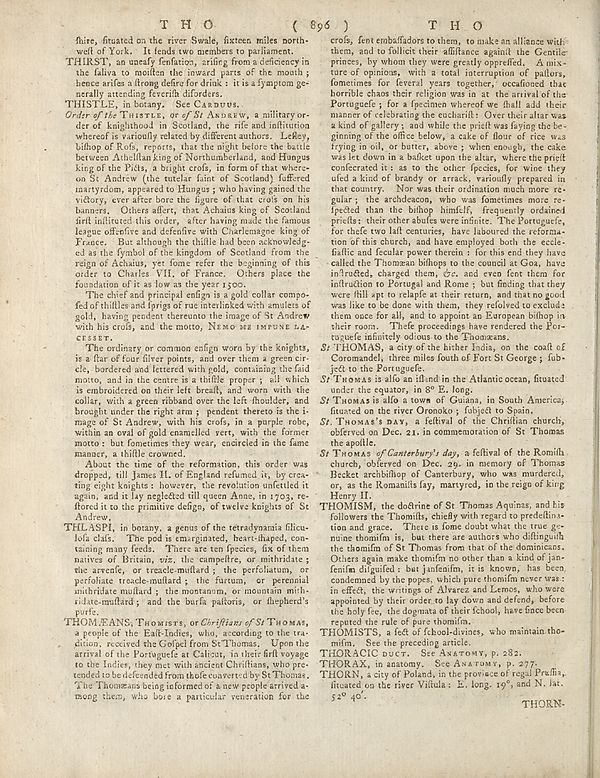
\includegraphics[width=0.85\textwidth]{../scans/page-1614-ea352b487d65.jpg}
\caption*{Source scan: \texttt{page-1614-ea352b487d65.jpg}}
\end{figure}

\end{document}
